%-------------------------------------------------
% FileName: chapt-3.tex
% Author: MrLQQ
% Date: 2021-10-7
% Description: 第3章
% Others: 
% History: origin
%------------------------------------------------- 

% 断页
% \clearpage 

\chapter{需求分析}

\section{功能需求分析}
% 引用图片的例子
描述系统的功能性需求,可以通过数据流图或UML的用例图等图表工具来部来定义系统的功能需求,并把需求和设计完全分离开。如图\ref{fig:single}所示。

% xelatex 支持的图片格式
% 矢量图 .pdf .eps 
% 位图 .jpg .png .bmp

% figure环境
% [H] 浮动优先级,当前位置,但尺寸过大的浮动体可能使得分页比较困难

% [htbp!] 浮动方式 请参考一份(不太)简短的 LATEX 2" 介绍,3.9节
% h 当前位置(代码所处的上下文)
% t 顶部
% b 底部
% p 单独成页
% ! 在决定位置时忽视限制
% 排版位置的选取与参数里符号的顺序无关, 
% LATEX 总是以 h-t-b-p 的优先级顺序决定浮动体位置。
% 也就是说 [!htp] 和 [ph!t] 没有区别。

\begin{figure}[H]
	% 居中
	\centering 
	% width=.5\textwidth 文档宽度的0.5
	% fig1图片放在img目录下,在此处引用无需img/前缀和图片格式后缀(png, jpg等)
	
\includegraphics[width=.5\textwidth]{fig1} 
	% label紧接caption之后,用于引用
	\caption{这是一个很长很长的图的名字图的名字图的名字图的名字图的名字图的名字图的名字图的名字图的名字图的名字图的名字图的名字图的名字图的名字图的名字图的名字图的名字图的名字图的名字图的名字图的名字图的名字图的名字图的名字图的名字图的名字图的名字图的名字图的名字图的名字图的名字图的名字图的名字图的名字图的名字}
	\label{fig:single}
\end{figure}


\section{系统业务分析}
如图\ref{fig:double}所示。

% 两个图并排
\begin{figure}[H]
	\centering
    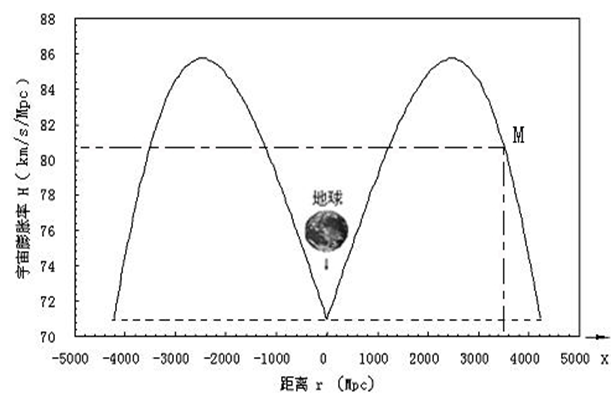
\includegraphics[width=.4\textwidth]{fig2}
    \quad % 横向两图的间距
    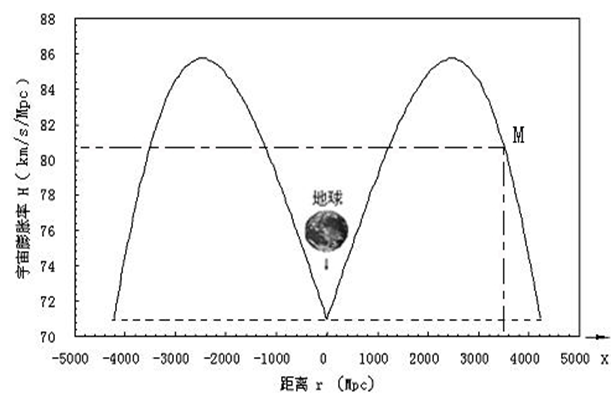
\includegraphics[width=.4\textwidth]{fig2} 
	\caption{两个图}
	\label{fig:double}
\end{figure}

\section{系统用例分析}

如图\ref{fig:fourimg}所示。

% 四个图并排
\begin{figure}[H]
	\centering
    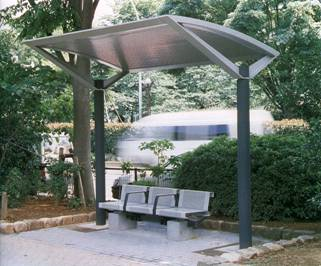
\includegraphics[width=.4\textwidth]{fig3}
    \quad 
	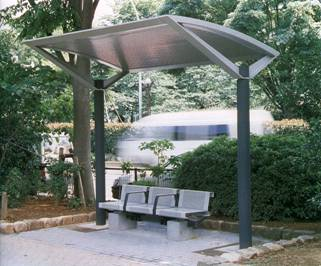
\includegraphics[width=.4\textwidth]{fig3} 
	% 空一行,分两行排版

	% 垂直间距 ex当前字号下小写字母 x 的高度
	\vspace{1ex} 
	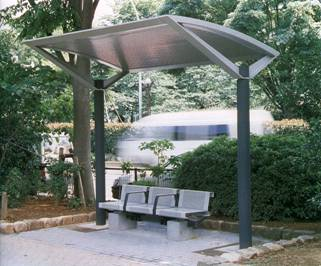
\includegraphics[width=.4\textwidth]{fig3}
	\quad
	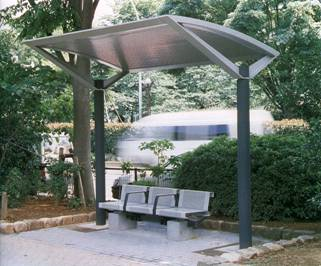
\includegraphics[width=.4\textwidth]{fig3}
	\caption{四个图}
	\label{fig:fourimg}
\end{figure}

\section{系统功能分析}

% % tikz绘图
% % 参考文档 texdoc tikz

% \begin{figure}[H]
% 	\centering
% 	\begin{tikzpicture}
% 		\begin{scope}[canvas is zy plane at x=0]
% 		\draw (0,0) circle (1cm);
% 		\draw (-1,0) -- (1,0) (0,-1) -- (0,1);
% 		\end{scope}
% 		\begin{scope}[canvas is zx plane at y=0]
% 		\draw (0,0) circle (1cm);
% 		\draw (-1,0) -- (1,0) (0,-1) -- (0,1);
% 		\end{scope}
% 		\begin{scope}[canvas is xy plane at z=0]
% 		\draw (0,0) circle (1cm);
% 		\draw (-1,0) -- (1,0) (0,-1) -- (0,1);
% 		\end{scope}
% 	\end{tikzpicture}
% 	\caption{画个圈圈}\label{fig:tikzcircle}
% \end{figure}

% \begin{figure}[H]
% 	\centering
% 	\begin{tikzpicture} 
% 		\draw[-stealth,line width=0.2pt] (-0.5,0) -- (4.5,0);
% 		\draw[-stealth,line width=0.2pt] (0,-0.5) -- (0,2.5);
% 		\coordinate (a) at (0.5,1.9);
% 		\coordinate (b) at (4,1.2);
% 		\node[below] (a0) at (a |- 0,0) {$a$};
% 		\node[below] (b0) at (b |- 0,0) {$b$};
% 		\filldraw[fill=gray!20,draw,thick]
% 		(a0) -- (a) .. controls (1,2.8) and (2.7,0.4) .. (b) -- (b0) -- cycle;
% 		\node[above right,outer sep=0.2cm, rounded corners,
% 		fill=green!20,draw=gray,text=blue!60!black,scale=0.6]
% 		at (b) {$\displaystyle \int_a^b {f(x)\,\mathrm{d}x} = F(b) - F(a)$}; 
% 	\end{tikzpicture}
% 	\caption{画个曲线}\label{fig:tikzcurve}
% \end{figure}


% \begin{figure}[H]
% 	\centering
% 	\tikz \graph [tree layout, nodes={draw,circle}, sibling sep=0pt]{ r -> { a, , ,b -> {c,d}, ,e} };
% 	\caption{画个树}\label{fig:tikztree}
% \end{figure}


\section{非功能需求分析}
描述系统的一些非功能方面的需求,如开发和运行环境、性能、人机交互、用户体验等。
 
 


 